\documentclass{beamer}
\usepackage[T1]{fontenc}
\usepackage[utf8]{inputenc}
\usepackage[ngerman,english,dutch,strings]{babel}
\usepackage{latexsym} 
\usepackage{amsfonts} 
\usepackage{amsmath}
\usepackage{amssymb}
\usepackage{amsthm}
\usepackage{beamerthemesplit}
\usecolortheme{beaver}
\usepackage{bbm}


\AtBeginSection[]{
  \begin{frame}
  \vfill
  \centering
  \begin{beamercolorbox}[sep=8pt,center,shadow=true,rounded=true]{title}
    \usebeamerfont{title}\insertsectionhead\par%
  \end{beamercolorbox}
  \vfill
  \end{frame}
}

\title{Binäre Klassifikation mit Python}
\author{Lennart Duvenbeck, Adrian Schoch, Markus Duong}
\date{25.07.2019}

\begin{document}
\maketitle
\begin{frame}{Inhaltsverzeichnis}
  \tableofcontents
\end{frame}


\section{Verfahren und Aufgabenstellung}

\subsection{Verfahren}
\begin{frame}
Gegeben: 
\begin{description}
\item[1.] Trainings-Datensatz D
\item[2.] Test-Datensatz $D^{'}$
\item[3.] eine Menge möglicher k: K
\item[4.] $l \in \mathbb{N}$ 
\end{description}
Gesucht: resultierender Klassifikator: 
\[
f_ {D} := \text{sign} \bigg( \sum_{i=1}^{l} f_{D_{\textbackslash i}, k^{*}}\bigg)
\]
Also: Bestimme das optimale $k^* \in K$
\end{frame}



\begin{frame}
Zerlegen des Datensatzes in l etwa gleichgroße Teildatensätze:
\[
D= D_1 \cup D_2 \cup ... \cup D_l
\]
Definition der "Komplemente":
\[
D_{\textbackslash i} := D_{1} \cup ... \cup D_{i-1} \cup D_{i+1} \cup...\cup D_{l}
\]
\end{frame}


\begin{frame}
Betrachte nun jedes mögliche k:\\
Berechne Klassifikationsfehlerrraten:
\[ \mathcal{R}_{D_i}(f_{D \textbackslash i ,k})= \frac{1}{m_i} \sum_{j=1}^{m_i} \mathbbm{1}_{y_{j}' \neq f_{D \textbackslash i ,k}(x_{j}')}
\]
Wobei $m_i$ die Anzahl der Punkte in $D_i$ ist und $f_{D \textbackslash i ,k}(x)$ die Klassifikationsfunktion
\[f_{D \textbackslash i ,k}(x) = \text{sign} \bigg( \sum_{j =1}^{k} y_{i_{j}}\bigg)
\]
Die $y_{i_j}$ sind dabei die Klassifikationen der k nächsten Nachbarn 
$x_{i_1},....,x_{i_k}$ von x in $D \textbackslash i$
\end{frame}

\begin{frame}
Nun erhält man $k^*$: 
\[k^* = argmin_{k \in K} \frac{1}{l} \sum_{i=1}^l \mathcal{R}_{D_i}(f_{D \textbackslash i ,k})
\]
Und der Klassifikator ist:
\[f_ {D} := \text{sign} \bigg( \sum_{i=1}^{l} f_{D_{\textbackslash i}, k^{*}}\bigg)
\]
\end{frame}

\subsection{Aufgabenstellung}
\begin{frame}
Ziel: classify-Funktion\\
Input: name, Kset, l \\
Output: name.result.csv, Klassifikationsfehlerrate $\mathcal{R}_{D'}(f_{D})$ \\
\vspace{20 mm}
\center{\Huge{EFFIZIENT}}
\end{frame}



\section{Implementierung}




\subsection{Erstes lauffähiges Programm}

\begin{frame}[fragile]
Importieren aller nötiger Funktionen
\begin{verbatim}
import numpy as np
from file_import import file_import
from nearest_points import nearest_points_naive_l1

def classify(name, KSET, l):
\end{verbatim}
\end{frame}

\begin{frame}[fragile]
Importieren der Datensätze\\
Feststellen der Dimension und Punktanzahl\\
Anlegen leerer Arrays, die noch benötigt werden\\
\begin{verbatim}
k_max = max(KSET)
test = file_import(name + ".test.csv")  
train = file_import(name + ".train.csv")  
n = train.shape[0]  
m = train.shape[1] 
index_array = np.zeros((n, k_max), dtype=int)  
block_size = n // l  
D_i_array = np.zeros((l, block_size, m))  
D_strich_i_array = np.zeros((l, block_size * (l - 1), m))  
\end{verbatim}
\end{frame}

\begin{frame}[fragile]
Anlegen der Teildatensätze für i=1,...,l in 3D-Arrays
\begin{verbatim}
for i in range(l):
        D_i_array[i] = 
        train[i * block_size:(i + 1) * block_size, :]
        lower_points = 
        train[0:i * block_size, :]
        upper_points = 
        train[(i + 1) * block_size:l * block_size, :]
        D_strich_i_array[i] =
        np.vstack((lower_points, upper_points))
\end{verbatim}
Laufzeit für bananas-1-2d:
\begin{verbatim}
0.0323243141 seconds
\end{verbatim}
\end{frame}

\begin{frame}[fragile]
Bestimmen der nächsten Nachbarn
\begin{verbatim}
for i in range(l):
        for j in range(0, block_size):
            index_array[block_size * i + j, :] =
            nearest_points_naive_l1(
            D_i_array[i, j, :],
            D_strich_i_array[i, :, :], 
            k_max)
\end{verbatim}
Laufzeit für bananas-1-2d:
\begin{verbatim}
6.1040873528 seconds
\end{verbatim}
\end{frame}

\begin{frame}[fragile]
Grobe Struktur zum Bestimmen des $k^*$
\begin{verbatim}
for k in KSET:
        Code
        for i in range(l):
            Code
            for j in range(0, block_size):
                Code
            Code
        Code
\end{verbatim}
\end{frame}

\begin{frame}[fragile]
Anlegen der benötigten Arrays
\begin{verbatim}
for k in KSET:
     errorarray = np.zeros(l)
     for i in range(l):
          C_i = np.zeros(block_size)
          for j in range(0, block_size):
\end{verbatim}
\end{frame}

\begin{frame}[fragile]
Berechnen der Klassifikationsfunktion für die einzelnen Punkte\\
Hier i, k fest:
\begin{verbatim}
for j in range(0, block_size):
           temp = np.sign(np.sum(D_strich_i_array
           [i, index_array[i * block_size + j, :k], 0]))
           if temp == 0:
              temp = 1 #da sgn(0)=1 gelten soll
           if D_i_array[i, j, 0] == temp:
               c = 0
           else:
               c = 1
           C_i[j] = c
\end{verbatim}
\end{frame}


\begin{frame}[fragile]
Bestimmen des Mittelwertes der Fehlerklassifikationsrate für die einzelnen k\\
Bestimmen des optimalen k
\begin{verbatim}    	   errorarray[i] = sum(C_i) / block_size
   middle_k = (1 / l) * sum(errorarray)
   list_ks.append(middle_k)
k_stern = np.int(list_ks.index(min(list_ks)))
\end{verbatim}
Laufzeit für bananas-1-2d:
\begin{verbatim}
13.5280859470 seconds
\end{verbatim}
\end{frame}

\begin{frame}[fragile]
Bestimmen der $k^*$-nächsten Nachbarn aller Punkte aus dem Testdatensatz
\begin{verbatim}
o = len(test)
test_classification = np.zeros(o)
test_index_array = np.zeros((l, o, k_stern), dtype = int)
for i in range(l):
     for j in range(o):
          test_index_array[i, j, :] =
          nearest_points_naive_l1(
          test[j, :], D_strich_i_array[i, :, :], k_stern)
\end{verbatim}
Laufzeit für bananas-1-2d:
\begin{verbatim}
12.6847841740 seconds
\end{verbatim}
\end{frame}

\begin{frame}[fragile]
Bestimmen der Klassifikationen
\begin{verbatim}
for j in range(o):
     temp = 0
     for i in range(l):
         temp1 = D_strich_i_array[
                 i, test_index_array[i, j, :], 0]
         temp2 = np.sum(temp1)
         temp += np.sign(temp2)
         if np.sign(np.sum(
              D_strich_i_array
              [i, test_index_array[i, j, :]])) == 0:
              temp += 1
        test_classification[j] = np.sign(temp)
test[:,0]=test_classification
\end{verbatim}
\end{frame}

\begin{frame}[fragile]
Laufzeit für diesen Teil des Programms:
\begin{verbatim}
0.3436388969 seconds
\end{verbatim}
Die gesamte Laufzeit des Programms beträgt:
\begin{verbatim}
32.2712738514 seconds
\end{verbatim}
Hauptteil der Zeit:
\begin{description}
\item[1.] Suche der nächsten Nachbarn: 18-19 Sekunden
\item[2.] Bestimmen des optimalen k: 13-14 Sekunden
\end{description}
\end{frame}


\subsection{Erste Optimierung}

\begin{frame}[fragile]
Optimierung der Punktsuche:\\
Theoretische Vorüberlegung:
In der Aufgabenstellung: KEINE Normvorgabe\\
Sei $ x \in \mathbb{R} ^n$:\\
Möglichkeiten:
\begin{description}
\item[1.] $L^1-Norm$: $\Vert x\Vert _{1}= \sum_{i=1}^n |x_i| $
\item[2.] $L^2-Norm$:  $\Vert x\Vert _{2}=\sqrt{ \sum_{i=1}^n x_i ^2} $
\item[3.] $L^{\infty}-Norm$:  $\Vert x\Vert {\infty}= \max(x_1,....,x_n)$
\end{description}
2. Möglichkeit sehr schlecht, da viele Operationen.\\
Noch 1. und 3. Möglichkeit zur Wahl
\end{frame}


\begin{frame}[fragile]
Erste Implementierung der $L^1$-Norm:
\begin{verbatim}
def nearest_points_naive_l1(x, D, k):
    n = D.shape[0]
    D = D[:, 1:]
    x = x[1:]
    if k > n:
        k = n  
        warnings.warn("Anzahl
        gesuchter nächster Punkte ist größer als
        Anzahl verfügbarer Punkte")
    E = np.sum(np.abs(x - D), 1)
    I = np.argsort(E)
    return I[:k]
\end{verbatim}
\end{frame}



\begin{frame}[fragile]
Erste Implementierung der $L^{\infty}-Norm$:
\begin{verbatim}
def nearest_points_naive_sup(x, D, k):
   n = D.shape[0]
   D = D[:, 1:]
   x = x[1:]
   if k > n:
       k = n 
       warnings.warn("Anzahl
       gesuchter nächster Punkte ist größer als 
        Anzahl verfügbarer Punkte")
    E = np.max(np.abs(x - D), 1)
    I = np.argsort(E)
    return I[:k]
\end{verbatim} 
\end{frame}

\begin{frame}[fragile]
Optimierte Implementierung der $L^1$-Norm:
\begin{verbatim}
def nearest_points_opt_l1(x, D, k):
    n = D.shape[0]
    D = D[:, 1:]
    x = x[1:]
    if k > n:
        k = n  
        warnings.warn("Anzahl
        gesuchter nächster Punkte ist größer als
        Anzahl verfügbarer Punkte")
    E = np.sum(np.abs(x - D), 1)
    P = np.argpartition(E, k)[:k]
    map = dict(zip(E[P], P))
    I = np.sort(E[P])
    return np.array([map[i] for i in I])
\end{verbatim}
\end{frame}

\begin{frame}[fragile]
Optimierte Implementierung der $L^{\infty}$-Norm:
\begin{verbatim}
def nearest_points_opt_sup(x, D, k):
    n = D.shape[0]
    D = D[:, 1:]
    x = x[1:]
    if k > n:
        k = n 
        warnings.warn("Anzahl 
        gesuchter nächster Punkte ist größer als Anzahl verfügbarer Punkte")
    E = np.max(np.abs(x - D), 1)
    if k == 0:
        return np.argmin(E)
    P = np.argpartition(E, k)[:k]
    map = dict(zip(E[P], P))
    I = np.sort(E[P])
    return np.array([map[i] for i in I])
\end{verbatim}
\end{frame}

\begin{frame}
Rechenaufwand der verwendeten Operationen:\\
np.argsort: $O(n*log(n))$\\
np.argpartition: $O(log(n))$\\
Vergleich der präsentierten Methoden und eines KD-Baumes aus der scipy-Bibliothek.
Wähle einen Datensatz aus und bestimme für jeden Punkt aus dem Datensatz die 200 nächsten Nachbarn.
\end{frame}

\begin{frame}[fragile]
1. Datensatz: toy-2d.train.csv: 10499 2D-Punkte
\begin{verbatim}
l1-naiv : 8.6845529079 seconds
lsup-naiv : 7.7315573692 seconds
l1-opt : 4.3814079762 seconds
lsup-opt : 3.4447133541 seconds
l1-kdt : 11.5258677006 seconds
lsup-kdt : 9.9952528477 seconds
\end{verbatim}
\end{frame}

\begin{frame}[fragile]
2. Datensatz: toy-4d.train.csv: 10499 4D-Punkte
\begin{verbatim}
l1-naiv : 9.2204573154 seconds
lsup-naiv : 9.9663882256 seconds
l1-opt : 4.7280640602 seconds
lsup-opt : 5.7798974514 seconds
l1-kdt : 20.4842510223 seconds
lsup-kdt : 15.4026172161 seconds
\end{verbatim}
\end{frame}

\begin{frame}[fragile]
3. Datensatz: toy-10d.train.csv: 10499 10D-Punkte
\begin{verbatim}
l1-naiv : 11.3101446629 seconds
lsup-naiv : 12.4345607758 seconds
l1-opt : 6.1001124382 seconds
lsup-opt : 7.9787714481 seconds
l1-kdt : 45.2455954552 seconds
lsup-kdt : 26.2906966209 seconds
\end{verbatim}
\end{frame}

\begin{frame}[fragile]
4. Datensatz: ijcnn1.10000.train.csv: 6999 
22D-Punkte
\begin{verbatim}
l1-naiv : 13.6359348297 seconds
lsup-naiv : 11.8157382011 seconds
l1-opt : 11.5597970486 seconds
lsup-opt : 12.1790583134 seconds
l1-kdt : 74.1918091774 seconds
lsup-kdt : 34.1802322865 seconds
\end{verbatim}
\end{frame}


\begin{frame}
Die optimierten Varianten sind für beide Normen besser als die naive Methode und der KD-Baum.\\
Bei höheren Dimensionen werden die Unterschiede zwischen der naiven Version und der optimierten Version kleiner.\\
Für den vorhin betrachteten Datensatz bananas-1-2d ergibt sich:
Laufzeit zuvor: 18-19 Sekunden\\
Laufzeit danach: 9-10 Sekunden
\end{frame}

\subsection{Zweite Optimierung}

\begin{frame}[fragile]
Nun: Optimierung der Berechnung des $k^*$\\
Stand des Programms vor der Optimierung
\begin{verbatim}
for k in KSET:
        Code
        for i in range(l):
            Code
            for j in range(0, block_size):
                Code
            Code
        Code
\end{verbatim}
Optimierung der vielen Schleifen durch Vektorisierung
\end{frame}

\begin{frame}[fragile]
Bestimmen der Klassifikatorfunktionen
\begin{verbatim}
new_array = np.zeros((l, block_size, k_max))  
for i in range(l):
   for j in range(block_size):
       new_array[i, j, :] = np.cumsum(
       D_strich_i_array[
       i,index_array[i * block_size + j, :], 0])
temp1_array = np.sign(new_array)
temp2_array = np.zeros((l, block_size, k_max))
\end{verbatim}
\end{frame}


\begin{frame}[fragile]
Bestimmung der Fehlerklassifikationen für die verschiedenen k\\
Bestimmung des $k^*$
\begin{verbatim}
for i in range(l):
     for j in range(block_size):
         for k in range(len(KSET)):
             if temp1_array[i, j, k] == 0:
                 temp1_array[i, j, k] = 1
             if D_i_array[i, j, 0] == temp1_array[i, j, k]:
                 temp2_array[i, j, k] = 0
             else:
                 temp2_array[i, j, k] = 1
temp3_array = np.sum(temp2_array, 1) / block_size
temp4_array = np.sum(temp3_array, 0) / l
k_stern = np.argmin(temp4_array)
\end{verbatim}
Laufzeit zuvor: 13-14 Sekunden\\
Laufzeit danach: 1.5-2 Sekunden
\end{frame}

\subsection{Zusammenfassung der Optimierung}
\begin{frame}[fragile]
Laufzeit für bananas-1-2d vor der Optimierung:
\begin{verbatim}
32.2712738514 seconds
\end{verbatim}
Laufzeit für bananas-1-2d nach der Optimierung:
\begin{verbatim}
11.6222813129 seconds
\end{verbatim}
Neue Laufzeit beträgt ca. 35\% der vorherigen Laufzeit
\end{frame}

\begin{frame}[fragile]
Laufzeit für toy-2d vor der Optimierung:
\begin{verbatim}
36.3387167454 seconds
\end{verbatim}
Laufzeit für toy-2d nach der Optimierung:
\begin{verbatim}
12.4756846428 seconds
\end{verbatim}
Neue Laufzeit beträgt ca. 33\% der vorherigen Laufzeit
\end{frame}

\begin{frame}[fragile]
Laufzeit für toy-4d vor der Optimierung:
\begin{verbatim}
37.2763948441 seconds
\end{verbatim}
Laufzeit für toy-4d nach der Optimierung:
\begin{verbatim}
13.8579912186 seconds
\end{verbatim}
Neue Laufzeit beträgt ca. 38\% der vorherigen Laufzeit
\end{frame}


\begin{frame}[fragile]
Laufzeit für toy-10d vor der Optimierung:
\begin{verbatim}
40.4189629555 seconds
\end{verbatim}
Laufzeit für toy-10d nach der Optimierung:
\begin{verbatim}
17.4822709560 seconds
\end{verbatim}
Neue Laufzeit beträgt ca. 43\% der vorherigen Laufzeit
\end{frame}

\begin{frame}[fragile]
Laufzeit für ijcnn1.10000 vor der Optimierung:
\begin{verbatim}
24.9962060452 seconds
\end{verbatim}
Laufzeit für ijcnn1.10000 nach der Optimierung:
\begin{verbatim}
11.8453524113 seconds
\end{verbatim}
Neue Laufzeit beträgt ca. 47\% der vorherigen Laufzeit
\end{frame}

\begin{frame}
Insgesamt deutliche Optimierung der Laufzeit.\\
Prozentual besten Verbesserungen bei kleineren Dimensionen
\end{frame}

\section{Grafische Darstellung}
\begin{figure}[h]
\centering
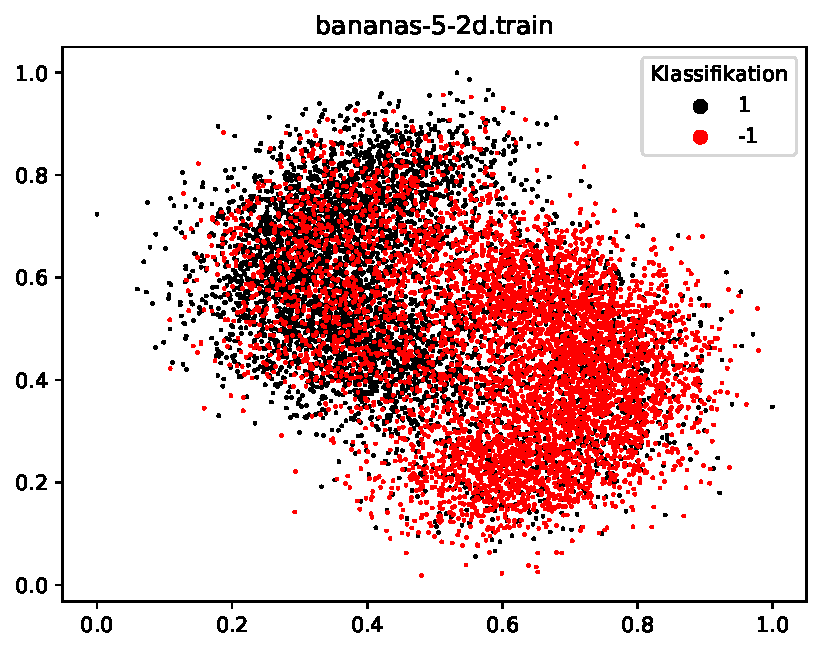
\includegraphics[scale=0.7]{bananas-5-2d-train.pdf}
\label{bananas}
\end{figure}

\begin{figure}[h]
\centering
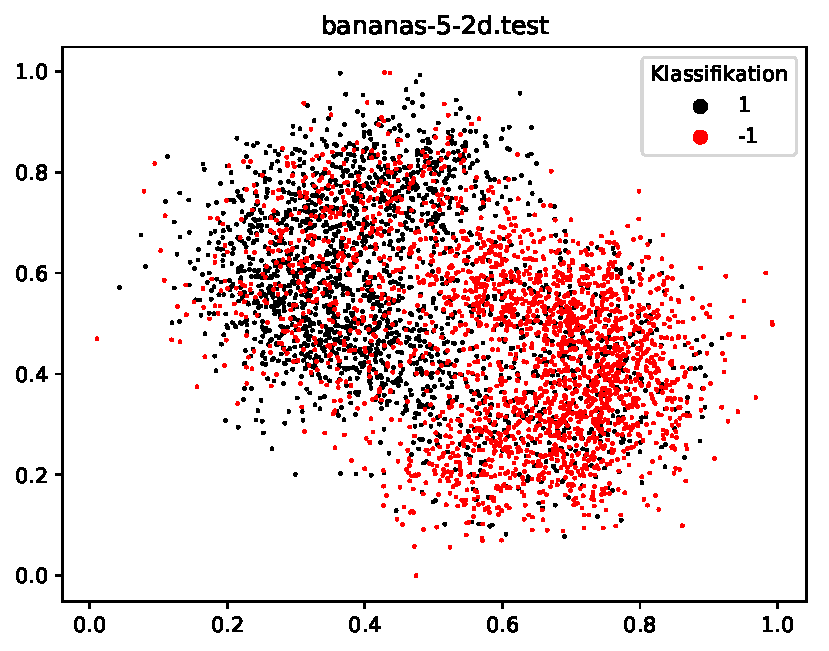
\includegraphics[scale=0.7]{bananas-5-2d-test.pdf}
\label{bananas}
\end{figure}

\begin{figure}[h]
\centering
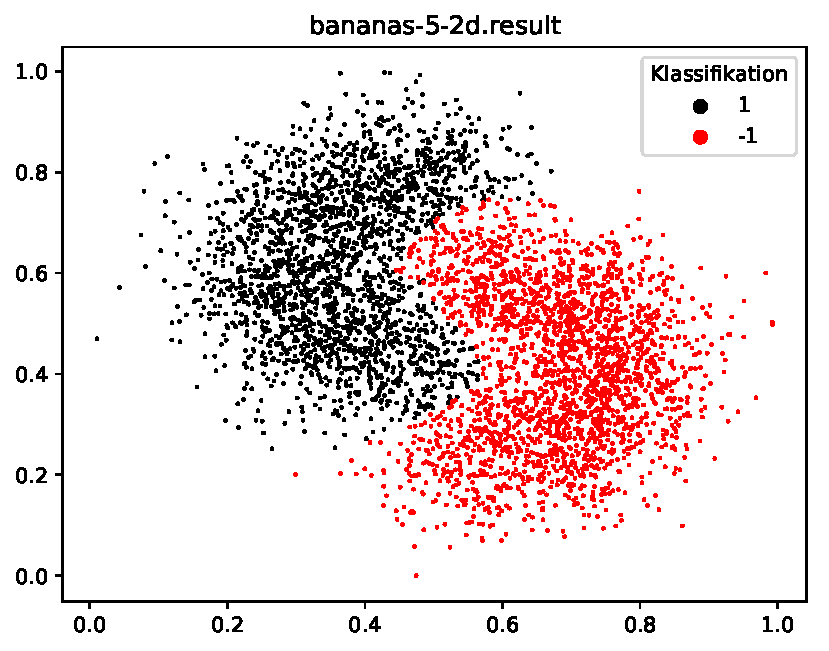
\includegraphics[scale=0.7]{bananas-5-2d-result.pdf}
\label{bananas}
\end{figure}

%Neuer Datensatz

\begin{figure}[h]
\centering
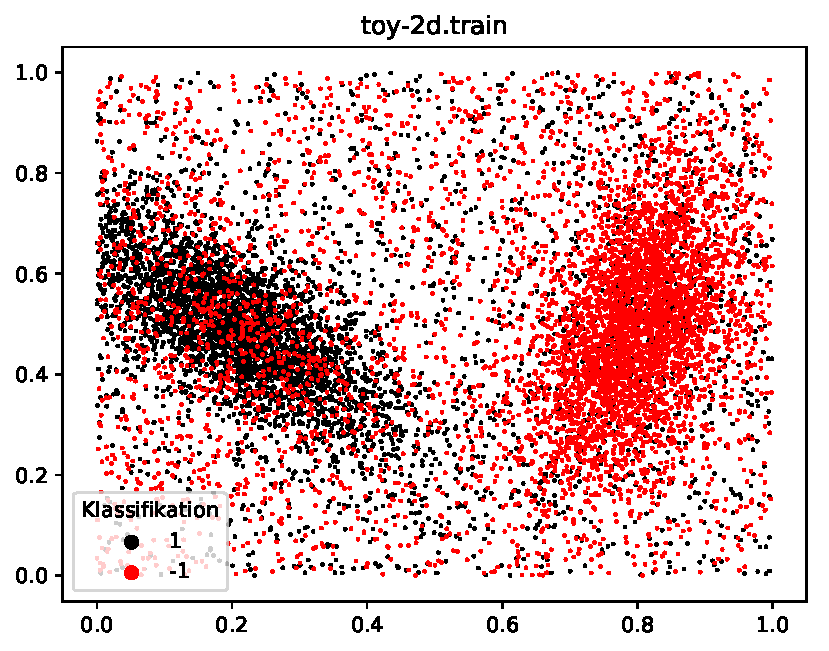
\includegraphics[scale=0.7]{toy-2d-train.pdf}
\label{bananas}
\end{figure}

\begin{figure}[h]
\centering
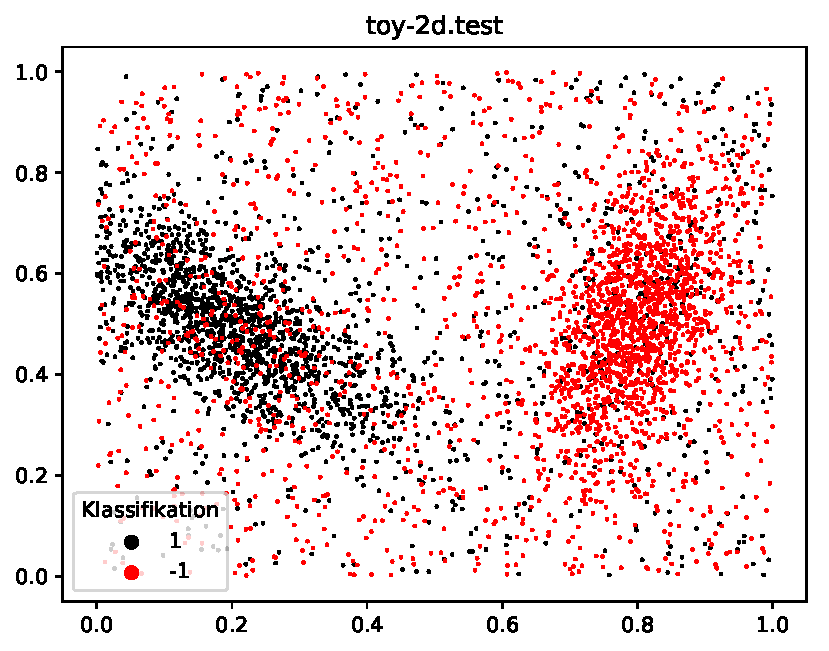
\includegraphics[scale=0.7]{toy-2d-test.pdf}
\label{bananas}
\end{figure}

\begin{figure}[h]
\centering
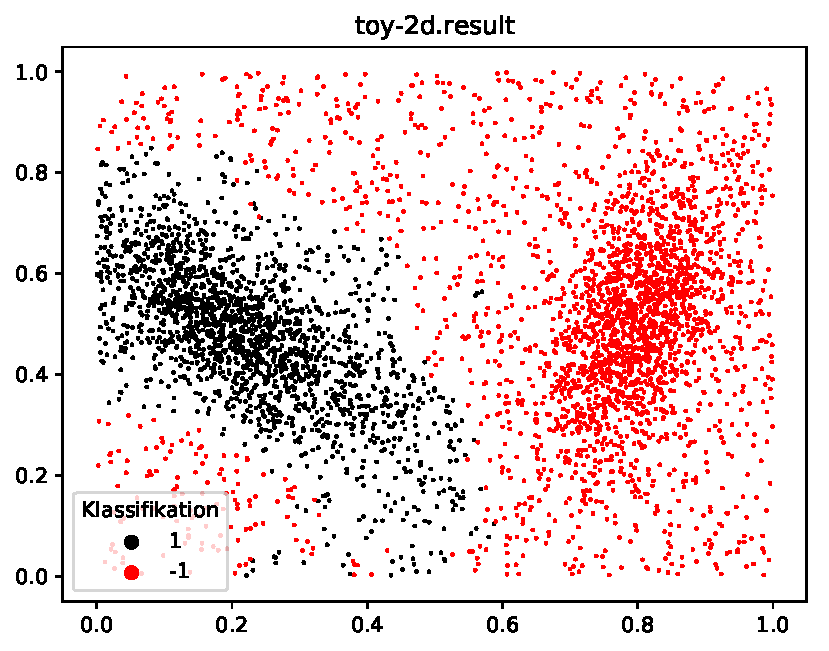
\includegraphics[scale=0.7]{toy-2d-result.pdf}
\label{bananas}
\end{figure}

\begin{frame}
\center{\Huge{Vielen Dank für Ihre}}
\center{\Huge{Aufmerksamkeit}}
\vspace{20mm}
\center{\huge{Gibt es noch Fragen ?}}
\end{frame}




\end{document}
